\PassOptionsToPackage{unicode=true}{hyperref} % options for packages loaded elsewhere
\PassOptionsToPackage{hyphens}{url}
%
\documentclass[]{article}
\usepackage{lmodern}
\usepackage{amssymb,amsmath}
\usepackage{ifxetex,ifluatex}
\usepackage{fixltx2e} % provides \textsubscript
\ifnum 0\ifxetex 1\fi\ifluatex 1\fi=0 % if pdftex
  \usepackage[T1]{fontenc}
  \usepackage[utf8]{inputenc}
  \usepackage{textcomp} % provides euro and other symbols
\else % if luatex or xelatex
  \usepackage{unicode-math}
  \defaultfontfeatures{Ligatures=TeX,Scale=MatchLowercase}
\fi
% use upquote if available, for straight quotes in verbatim environments
\IfFileExists{upquote.sty}{\usepackage{upquote}}{}
% use microtype if available
\IfFileExists{microtype.sty}{%
\usepackage[]{microtype}
\UseMicrotypeSet[protrusion]{basicmath} % disable protrusion for tt fonts
}{}
\IfFileExists{parskip.sty}{%
\usepackage{parskip}
}{% else
\setlength{\parindent}{0pt}
\setlength{\parskip}{6pt plus 2pt minus 1pt}
}
\usepackage{hyperref}
\hypersetup{
            pdftitle={STA 326 2.0 Programming and Data Analysis with R},
            pdfborder={0 0 0},
            breaklinks=true}
\urlstyle{same}  % don't use monospace font for urls
\usepackage[left=3cm,right=3cm,top=2cm,bottom=2cm]{geometry}
\usepackage{color}
\usepackage{fancyvrb}
\newcommand{\VerbBar}{|}
\newcommand{\VERB}{\Verb[commandchars=\\\{\}]}
\DefineVerbatimEnvironment{Highlighting}{Verbatim}{commandchars=\\\{\}}
% Add ',fontsize=\small' for more characters per line
\usepackage{framed}
\definecolor{shadecolor}{RGB}{248,248,248}
\newenvironment{Shaded}{\begin{snugshade}}{\end{snugshade}}
\newcommand{\AlertTok}[1]{\textcolor[rgb]{0.94,0.16,0.16}{#1}}
\newcommand{\AnnotationTok}[1]{\textcolor[rgb]{0.56,0.35,0.01}{\textbf{\textit{#1}}}}
\newcommand{\AttributeTok}[1]{\textcolor[rgb]{0.77,0.63,0.00}{#1}}
\newcommand{\BaseNTok}[1]{\textcolor[rgb]{0.00,0.00,0.81}{#1}}
\newcommand{\BuiltInTok}[1]{#1}
\newcommand{\CharTok}[1]{\textcolor[rgb]{0.31,0.60,0.02}{#1}}
\newcommand{\CommentTok}[1]{\textcolor[rgb]{0.56,0.35,0.01}{\textit{#1}}}
\newcommand{\CommentVarTok}[1]{\textcolor[rgb]{0.56,0.35,0.01}{\textbf{\textit{#1}}}}
\newcommand{\ConstantTok}[1]{\textcolor[rgb]{0.00,0.00,0.00}{#1}}
\newcommand{\ControlFlowTok}[1]{\textcolor[rgb]{0.13,0.29,0.53}{\textbf{#1}}}
\newcommand{\DataTypeTok}[1]{\textcolor[rgb]{0.13,0.29,0.53}{#1}}
\newcommand{\DecValTok}[1]{\textcolor[rgb]{0.00,0.00,0.81}{#1}}
\newcommand{\DocumentationTok}[1]{\textcolor[rgb]{0.56,0.35,0.01}{\textbf{\textit{#1}}}}
\newcommand{\ErrorTok}[1]{\textcolor[rgb]{0.64,0.00,0.00}{\textbf{#1}}}
\newcommand{\ExtensionTok}[1]{#1}
\newcommand{\FloatTok}[1]{\textcolor[rgb]{0.00,0.00,0.81}{#1}}
\newcommand{\FunctionTok}[1]{\textcolor[rgb]{0.00,0.00,0.00}{#1}}
\newcommand{\ImportTok}[1]{#1}
\newcommand{\InformationTok}[1]{\textcolor[rgb]{0.56,0.35,0.01}{\textbf{\textit{#1}}}}
\newcommand{\KeywordTok}[1]{\textcolor[rgb]{0.13,0.29,0.53}{\textbf{#1}}}
\newcommand{\NormalTok}[1]{#1}
\newcommand{\OperatorTok}[1]{\textcolor[rgb]{0.81,0.36,0.00}{\textbf{#1}}}
\newcommand{\OtherTok}[1]{\textcolor[rgb]{0.56,0.35,0.01}{#1}}
\newcommand{\PreprocessorTok}[1]{\textcolor[rgb]{0.56,0.35,0.01}{\textit{#1}}}
\newcommand{\RegionMarkerTok}[1]{#1}
\newcommand{\SpecialCharTok}[1]{\textcolor[rgb]{0.00,0.00,0.00}{#1}}
\newcommand{\SpecialStringTok}[1]{\textcolor[rgb]{0.31,0.60,0.02}{#1}}
\newcommand{\StringTok}[1]{\textcolor[rgb]{0.31,0.60,0.02}{#1}}
\newcommand{\VariableTok}[1]{\textcolor[rgb]{0.00,0.00,0.00}{#1}}
\newcommand{\VerbatimStringTok}[1]{\textcolor[rgb]{0.31,0.60,0.02}{#1}}
\newcommand{\WarningTok}[1]{\textcolor[rgb]{0.56,0.35,0.01}{\textbf{\textit{#1}}}}
\usepackage{graphicx,grffile}
\makeatletter
\def\maxwidth{\ifdim\Gin@nat@width>\linewidth\linewidth\else\Gin@nat@width\fi}
\def\maxheight{\ifdim\Gin@nat@height>\textheight\textheight\else\Gin@nat@height\fi}
\makeatother
% Scale images if necessary, so that they will not overflow the page
% margins by default, and it is still possible to overwrite the defaults
% using explicit options in \includegraphics[width, height, ...]{}
\setkeys{Gin}{width=\maxwidth,height=\maxheight,keepaspectratio}
\setlength{\emergencystretch}{3em}  % prevent overfull lines
\providecommand{\tightlist}{%
  \setlength{\itemsep}{0pt}\setlength{\parskip}{0pt}}
\setcounter{secnumdepth}{0}
% Redefines (sub)paragraphs to behave more like sections
\ifx\paragraph\undefined\else
\let\oldparagraph\paragraph
\renewcommand{\paragraph}[1]{\oldparagraph{#1}\mbox{}}
\fi
\ifx\subparagraph\undefined\else
\let\oldsubparagraph\subparagraph
\renewcommand{\subparagraph}[1]{\oldsubparagraph{#1}\mbox{}}
\fi

% set default figure placement to htbp
\makeatletter
\def\fps@figure{htbp}
\makeatother

\usepackage{etoolbox}
\makeatletter
\providecommand{\subtitle}[1]{% add subtitle to \maketitle
  \apptocmd{\@title}{\par {\large #1 \par}}{}{}
}
\makeatother

\title{STA 326 2.0 Programming and Data Analysis with R \footnote{All rights
  reserved by Thiyanga S. Talagala}}
\providecommand{\subtitle}[1]{}
\subtitle{Exploring \texttt{iris} dataset with \texttt{qplot}}
\author{}
\date{\vspace{-2.5em}31 March 2020}

\begin{document}
\maketitle

{
\setcounter{tocdepth}{3}
\tableofcontents
}
\newpage

\hypertarget{stage-1-planning-your-analysis}{%
\section{Stage 1: Planning your
analysis}\label{stage-1-planning-your-analysis}}

\hypertarget{step-1-dataset-overview-and-description}{%
\subsection{Step 1: Dataset overview and
description}\label{step-1-dataset-overview-and-description}}

Before we get started let's look at the data and plan a analysis.

\textbf{Load iris dataset}

\begin{Shaded}
\begin{Highlighting}[]
\KeywordTok{data}\NormalTok{(iris)}
\end{Highlighting}
\end{Shaded}

Here is a glimpse of the dataset.

\begin{Shaded}
\begin{Highlighting}[]
\KeywordTok{head}\NormalTok{(iris)}
\end{Highlighting}
\end{Shaded}

\begin{verbatim}
  Sepal.Length Sepal.Width Petal.Length Petal.Width Species
1          5.1         3.5          1.4         0.2  setosa
2          4.9         3.0          1.4         0.2  setosa
3          4.7         3.2          1.3         0.2  setosa
4          4.6         3.1          1.5         0.2  setosa
5          5.0         3.6          1.4         0.2  setosa
6          5.4         3.9          1.7         0.4  setosa
\end{verbatim}

We have four quantitative variables: Sepal.Length, Sepal.Width,
Petal.Length, Petal.Width and one qualitative variable: Species

\hypertarget{step-2-one-way-analysis}{%
\subsection{Step 2: One-way analysis}\label{step-2-one-way-analysis}}

Let's look at the graphs we could use to explore variables one by one.

Plots that could be used to to summarize qualitative variables

\begin{itemize}
\item
  Bar chart
\item
  Pie chart
\end{itemize}

Plots that could be used to to summarize quantitative variables

\begin{itemize}
\item
  Box and whisker plot
\item
  Histograms
\item
  Dot plots
\item
  Density plot
\item
  Stem and leaf displays
\end{itemize}

Note: Stem and leaf displays are best-suited for small to moderate
datasets, whereas others such as histograms and Box and whisker plots
are best-suited for large datasets. Box and whisker plots and histograms
are also good at depicting differences between distributions and
identifying outliers.

\hypertarget{step-3-two-way-analysis}{%
\subsection{Step 3: Two-way analysis}\label{step-3-two-way-analysis}}

Next, we will look at two variables at a time.

\begin{itemize}
\item
  Quantitative vs Quantitative: Scatter plots
\item
  Quantitative vs Qualitative: Box plots/ Histograms/ Dot plots/ Density
  plots with groups allow us to compare across different levels of the
  qualitative variable. \textbf{Faceting} can be used to generate the
  same plot for different levels of the qualitative variable.
\end{itemize}

\hypertarget{step-4-three-way-analysis}{%
\subsection{Step 4: Three-way
analysis}\label{step-4-three-way-analysis}}

Now, let's look at three variables at a time.

\begin{itemize}
\tightlist
\item
  Two quantitative variables and one qualitative variable: Scatter plot
  with different markers (eg: size, shapes, colours) for different
  levels of the qualitative variable.
\end{itemize}

\hypertarget{stage-2-getting-started-with-qplot-in-the-ggplot2-package.}{%
\section{\texorpdfstring{Stage 2: Getting started with \texttt{qplot()}
in the ggplot2
package.}{Stage 2: Getting started with qplot() in the ggplot2 package.}}\label{stage-2-getting-started-with-qplot-in-the-ggplot2-package.}}

Now we are going to use the \texttt{qplot} function to make some quick
plots. This section demonstrates how different graphs can be plotted for
various purposes using the \texttt{qplot}.

\hypertarget{recap-some-important-arguments-in-qplot}{%
\subsection{\texorpdfstring{Recap: some important arguments in
\texttt{qplot}}{Recap: some important arguments in qplot}}\label{recap-some-important-arguments-in-qplot}}

\begin{Shaded}
\begin{Highlighting}[]
\KeywordTok{qplot}\NormalTok{(}
\NormalTok{  x, }\CommentTok{# X variable}
\NormalTok{  y, }\CommentTok{# Y variable}
\NormalTok{  data, }\CommentTok{# name of the dataframe}
  \DataTypeTok{facets =} \OtherTok{NULL}\NormalTok{, }
  \DataTypeTok{margins =} \OtherTok{FALSE}\NormalTok{,}
  \DataTypeTok{geom =} \StringTok{"auto"}\NormalTok{,}
  \DataTypeTok{xlim =} \KeywordTok{c}\NormalTok{(}\OtherTok{NA}\NormalTok{, }\OtherTok{NA}\NormalTok{), }\CommentTok{# numeric vector of length 2 giving the x coordinates}
  \DataTypeTok{ylim =} \KeywordTok{c}\NormalTok{(}\OtherTok{NA}\NormalTok{, }\OtherTok{NA}\NormalTok{), }\CommentTok{# numeric vector of length 2 giving the 7 coordinates}
  \DataTypeTok{log =} \StringTok{""}\NormalTok{,}
  \DataTypeTok{main =} \OtherTok{NULL}\NormalTok{, }\CommentTok{# Figure title}
  \DataTypeTok{xlab =} \OtherTok{NULL}\NormalTok{, }\CommentTok{# X-axis title}
  \DataTypeTok{ylab =} \OtherTok{NULL}\NormalTok{, }\CommentTok{# Y-axis title}
  \DataTypeTok{asp =} \OtherTok{NA}\NormalTok{,}
  \DataTypeTok{stat =} \OtherTok{NULL}\NormalTok{,}
  \DataTypeTok{position =} \OtherTok{NULL}\NormalTok{,}
\NormalTok{)}
\end{Highlighting}
\end{Shaded}

\newpage

\hypertarget{one-way-analysis}{%
\subsection{One-way analysis}\label{one-way-analysis}}

\hypertarget{load-packages}{%
\subsubsection{Load packages}\label{load-packages}}

\begin{Shaded}
\begin{Highlighting}[]
\KeywordTok{library}\NormalTok{(ggplot2)}
\end{Highlighting}
\end{Shaded}

\hypertarget{summarizing-qualitative-variables}{%
\subsubsection{1. Summarizing qualitative
variables}\label{summarizing-qualitative-variables}}

\begin{Shaded}
\begin{Highlighting}[]
\KeywordTok{qplot}\NormalTok{(}\DataTypeTok{x =}\NormalTok{ Species, }\DataTypeTok{data =}\NormalTok{ iris, }\DataTypeTok{geom =} \StringTok{"bar"}\NormalTok{, }\DataTypeTok{ylab =} \StringTok{"Count"}\NormalTok{,}
      \DataTypeTok{main =} \StringTok{"Composition of Species"}\NormalTok{)}
\end{Highlighting}
\end{Shaded}

\begin{figure}
\centering
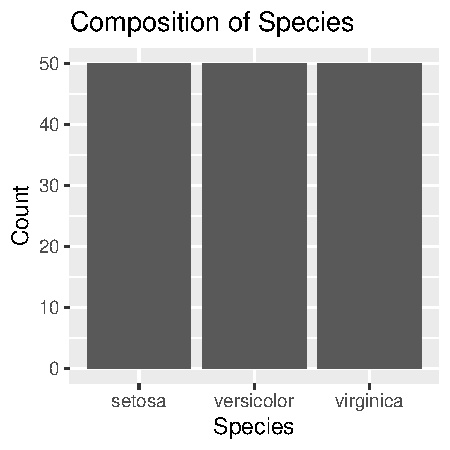
\includegraphics{Week3Answers_files/figure-latex/unnamed-chunk-4-1.pdf}
\caption{Composition of the sample}
\end{figure}

\newpage

\hypertarget{summarizing-quantitative-variables}{%
\subsubsection{2. Summarizing quantitative
variables}\label{summarizing-quantitative-variables}}

Here, I have drawn plots only for \texttt{Sepal.Width}. Please take
suitable graphs for other quantitative variables in the iris dataset.

\hypertarget{histogram}{%
\paragraph{Histogram}\label{histogram}}

\begin{Shaded}
\begin{Highlighting}[]
\KeywordTok{qplot}\NormalTok{(}\DataTypeTok{x =}\NormalTok{ Sepal.Width, }\DataTypeTok{data =}\NormalTok{ iris, }\DataTypeTok{geom =} \StringTok{"histogram"}\NormalTok{)}
\end{Highlighting}
\end{Shaded}

\begin{figure}
\centering
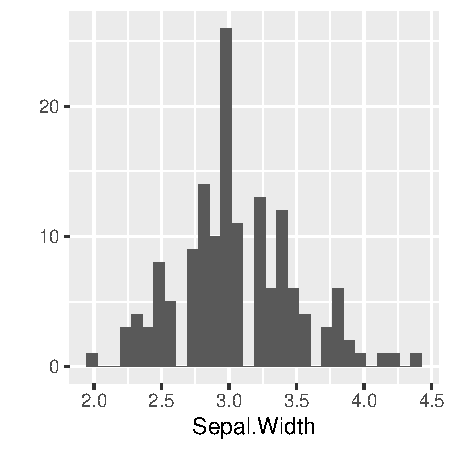
\includegraphics{Week3Answers_files/figure-latex/unnamed-chunk-5-1.pdf}
\caption{Histogram of sepal width}
\end{figure}

\hypertarget{density-plot}{%
\paragraph{Density plot}\label{density-plot}}

\begin{Shaded}
\begin{Highlighting}[]
\KeywordTok{qplot}\NormalTok{(}\DataTypeTok{x =}\NormalTok{ Sepal.Width, }\DataTypeTok{data =}\NormalTok{ iris, }\DataTypeTok{geom =} \StringTok{"density"}\NormalTok{)}
\end{Highlighting}
\end{Shaded}

\begin{figure}
\centering
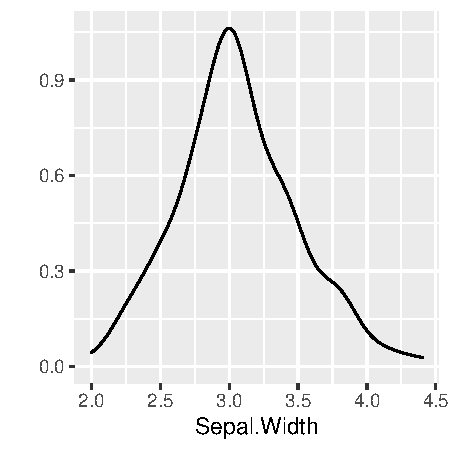
\includegraphics{Week3Answers_files/figure-latex/unnamed-chunk-6-1.pdf}
\caption{Density plot of sepal width}
\end{figure}

\newpage

\hypertarget{box-and-whisker-plot}{%
\paragraph{Box and whisker plot}\label{box-and-whisker-plot}}

\begin{Shaded}
\begin{Highlighting}[]
\KeywordTok{qplot}\NormalTok{(}\DataTypeTok{y =}\NormalTok{ Sepal.Width, }\DataTypeTok{data =}\NormalTok{ iris, }\DataTypeTok{geom =} \StringTok{"boxplot"}\NormalTok{)}
\end{Highlighting}
\end{Shaded}

\begin{figure}
\centering
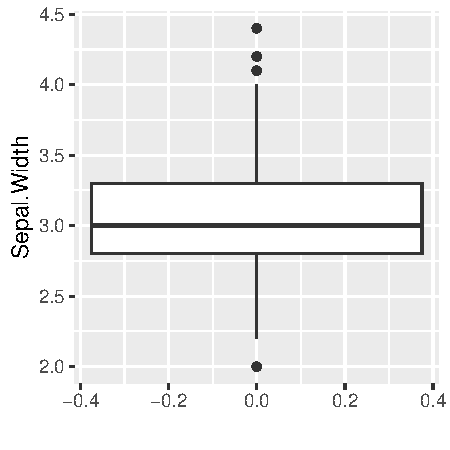
\includegraphics{Week3Answers_files/figure-latex/unnamed-chunk-7-1.pdf}
\caption{Boxplot of sepal width}
\end{figure}

\hypertarget{two-way-analysis}{%
\subsection{Two-way analysis}\label{two-way-analysis}}

\hypertarget{visualizing-two-qualitative-variables-at-a-time}{%
\subsubsection{1. Visualizing two qualitative variables at a
time}\label{visualizing-two-qualitative-variables-at-a-time}}

\begin{Shaded}
\begin{Highlighting}[]
\KeywordTok{qplot}\NormalTok{(}\DataTypeTok{x =}\NormalTok{ Sepal.Length, }\DataTypeTok{y =}\NormalTok{ Sepal.Width, }\DataTypeTok{data =}\NormalTok{ iris, }\DataTypeTok{geom =} \StringTok{"point"}\NormalTok{)}
\end{Highlighting}
\end{Shaded}

\begin{figure}
\centering
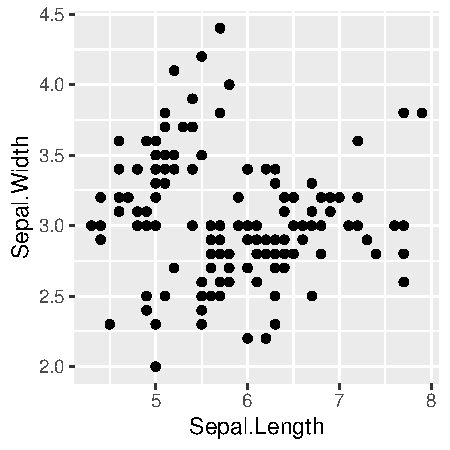
\includegraphics{Week3Answers_files/figure-latex/unnamed-chunk-8-1.pdf}
\caption{Scatterplot of sepal length and sepal width}
\end{figure}

\newpage

\hypertarget{visualizing-qualitative-and-quantitative-variables}{%
\subsubsection{2. Visualizing qualitative and quantitative
variables}\label{visualizing-qualitative-and-quantitative-variables}}

\begin{Shaded}
\begin{Highlighting}[]
\KeywordTok{qplot}\NormalTok{(}\DataTypeTok{x =}\NormalTok{ Species, }\DataTypeTok{y =}\NormalTok{ Sepal.Width, }\DataTypeTok{data =}\NormalTok{ iris, }\DataTypeTok{geom =} \StringTok{"boxplot"}\NormalTok{)}
\end{Highlighting}
\end{Shaded}

\begin{figure}
\centering
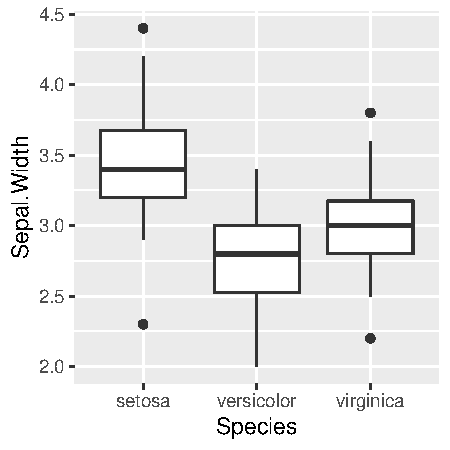
\includegraphics{Week3Answers_files/figure-latex/unnamed-chunk-9-1.pdf}
\caption{Boxplot of sepal width by species}
\end{figure}

\hypertarget{different-ways-to-modify-your-graph}{%
\paragraph{Different ways to modify your
graph}\label{different-ways-to-modify-your-graph}}

\begin{Shaded}
\begin{Highlighting}[]
\KeywordTok{qplot}\NormalTok{(}\DataTypeTok{x =}\NormalTok{ Species, }\DataTypeTok{y =}\NormalTok{ Sepal.Width, }\DataTypeTok{data =}\NormalTok{ iris, }\DataTypeTok{geom =} \StringTok{"boxplot"}\NormalTok{, }\DataTypeTok{fill =}\NormalTok{ Species)}
\end{Highlighting}
\end{Shaded}

\begin{figure}
\centering
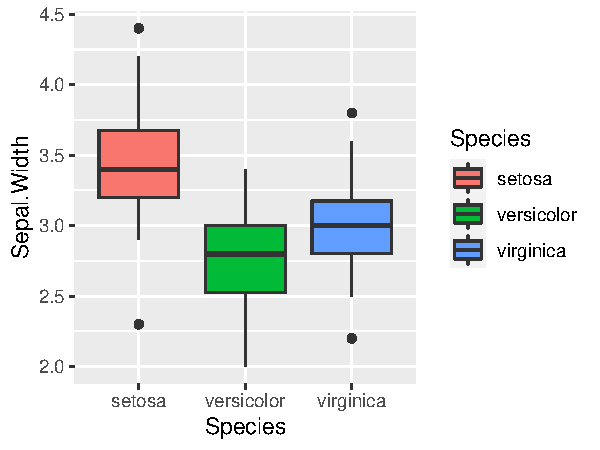
\includegraphics{Week3Answers_files/figure-latex/unnamed-chunk-10-1.pdf}
\caption{Boxplot of sepal width by species}
\end{figure}

\newpage

\begin{Shaded}
\begin{Highlighting}[]
\KeywordTok{qplot}\NormalTok{(}\DataTypeTok{x =}\NormalTok{ Species, }\DataTypeTok{y =}\NormalTok{ Sepal.Width, }\DataTypeTok{data =}\NormalTok{ iris, }\DataTypeTok{geom =} \KeywordTok{c}\NormalTok{(}\StringTok{"point"}\NormalTok{,}\StringTok{"jitter"}\NormalTok{,}\StringTok{"boxplot"}\NormalTok{), }
      \DataTypeTok{alpha =} \FloatTok{0.5}\NormalTok{, }\DataTypeTok{colour =}\NormalTok{ Species)}
\end{Highlighting}
\end{Shaded}

\begin{figure}
\centering
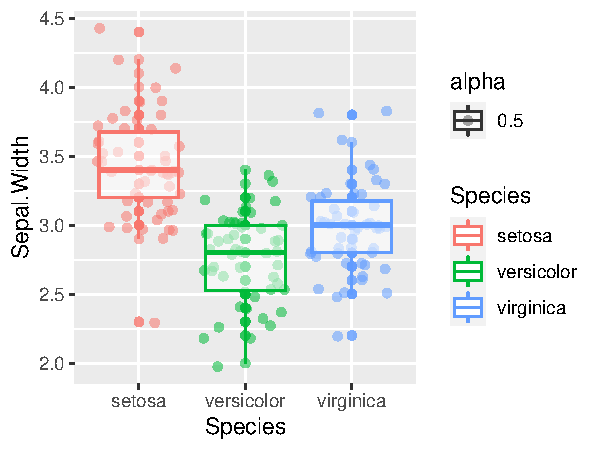
\includegraphics{Week3Answers_files/figure-latex/unnamed-chunk-11-1.pdf}
\caption{Boxplot of sepal width by species}
\end{figure}

\begin{Shaded}
\begin{Highlighting}[]
\KeywordTok{qplot}\NormalTok{(}\DataTypeTok{x =}\NormalTok{ Sepal.Width, }\DataTypeTok{data =}\NormalTok{ iris, }\DataTypeTok{geom =} \KeywordTok{c}\NormalTok{(}\StringTok{"histogram"}\NormalTok{), }
     \DataTypeTok{colour =}\NormalTok{ Species)}
\end{Highlighting}
\end{Shaded}

\begin{figure}
\centering
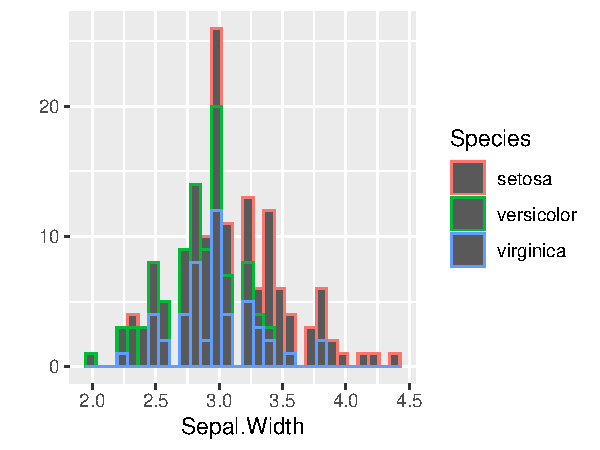
\includegraphics{Week3Answers_files/figure-latex/unnamed-chunk-12-1.pdf}
\caption{Histogram of sepal width}
\end{figure}

\newpage

\begin{Shaded}
\begin{Highlighting}[]
\KeywordTok{qplot}\NormalTok{(}\DataTypeTok{x =}\NormalTok{ Sepal.Width, }\DataTypeTok{data =}\NormalTok{ iris, }\DataTypeTok{geom =} \KeywordTok{c}\NormalTok{(}\StringTok{"histogram"}\NormalTok{), }
     \DataTypeTok{fill =}\NormalTok{ Species)}
\end{Highlighting}
\end{Shaded}

\begin{figure}
\centering
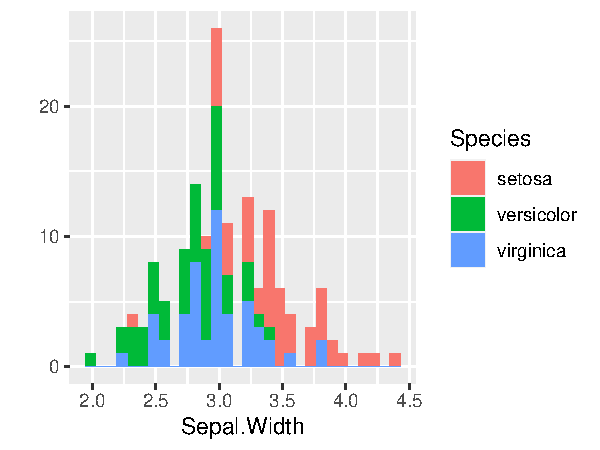
\includegraphics{Week3Answers_files/figure-latex/unnamed-chunk-13-1.pdf}
\caption{Histogram of sepal width}
\end{figure}

\begin{Shaded}
\begin{Highlighting}[]
\KeywordTok{qplot}\NormalTok{(}\DataTypeTok{x =}\NormalTok{ Sepal.Width, }\DataTypeTok{data =}\NormalTok{ iris, }\DataTypeTok{geom =} \KeywordTok{c}\NormalTok{(}\StringTok{"density"}\NormalTok{), }
     \DataTypeTok{colour =}\NormalTok{ Species)}
\end{Highlighting}
\end{Shaded}

\begin{figure}
\centering
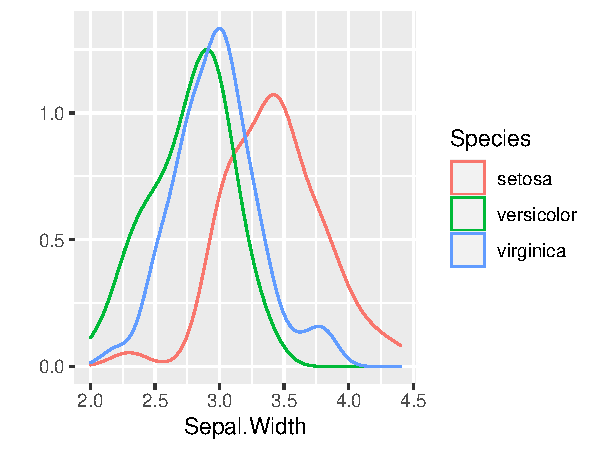
\includegraphics{Week3Answers_files/figure-latex/unnamed-chunk-14-1.pdf}
\caption{Density plot of sepal width}
\end{figure}

\newpage

\hypertarget{three-way-analysis}{%
\subsection{Three-way analysis}\label{three-way-analysis}}

\textbf{Everything on a single panel}

\begin{Shaded}
\begin{Highlighting}[]
\KeywordTok{qplot}\NormalTok{(}\DataTypeTok{x =}\NormalTok{ Sepal.Length, }\DataTypeTok{y =}\NormalTok{ Sepal.Width, }\DataTypeTok{data =}\NormalTok{ iris, }
      \DataTypeTok{geom =} \StringTok{"point"}\NormalTok{, }\DataTypeTok{color =}\NormalTok{ Species)}
\end{Highlighting}
\end{Shaded}

\begin{figure}
\centering
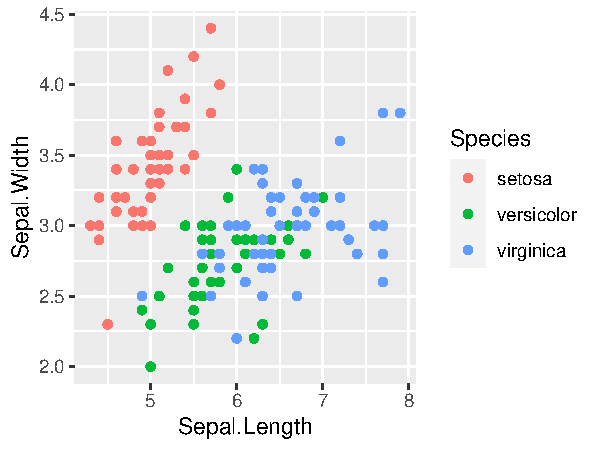
\includegraphics{Week3Answers_files/figure-latex/unnamed-chunk-15-1.pdf}
\caption{Scatterplot of sepal length and sepal width by species}
\end{figure}

\textbf{Separate panels for each species: column-wise}

\begin{Shaded}
\begin{Highlighting}[]
\KeywordTok{qplot}\NormalTok{(}\DataTypeTok{x =}\NormalTok{ Sepal.Length, }\DataTypeTok{y =}\NormalTok{ Sepal.Width, }
      \DataTypeTok{facets =}\NormalTok{ .}\OperatorTok{~}\NormalTok{Species, }\DataTypeTok{data =}\NormalTok{ iris, }\DataTypeTok{geom =} \StringTok{"point"}\NormalTok{) }
\end{Highlighting}
\end{Shaded}

\begin{figure}
\centering
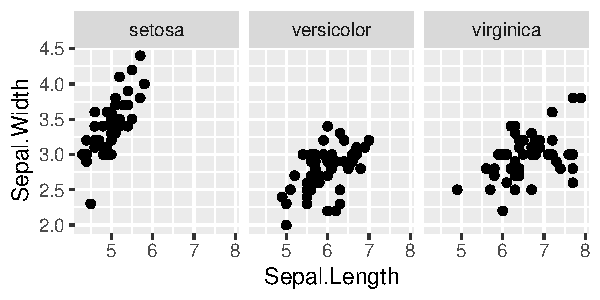
\includegraphics{Week3Answers_files/figure-latex/unnamed-chunk-16-1.pdf}
\caption{Scatterplot of sepal length and sepal width by species}
\end{figure}

\newpage

\textbf{Separate panels for each species: row-wise}

\begin{Shaded}
\begin{Highlighting}[]
\KeywordTok{qplot}\NormalTok{(}\DataTypeTok{x =}\NormalTok{ Sepal.Length, }\DataTypeTok{y =}\NormalTok{ Sepal.Width, }
      \DataTypeTok{facets =}\NormalTok{ Species}\OperatorTok{~}\NormalTok{., }\DataTypeTok{data =}\NormalTok{ iris, }\DataTypeTok{geom =} \StringTok{"point"}\NormalTok{)}
\end{Highlighting}
\end{Shaded}

\begin{figure}
\centering
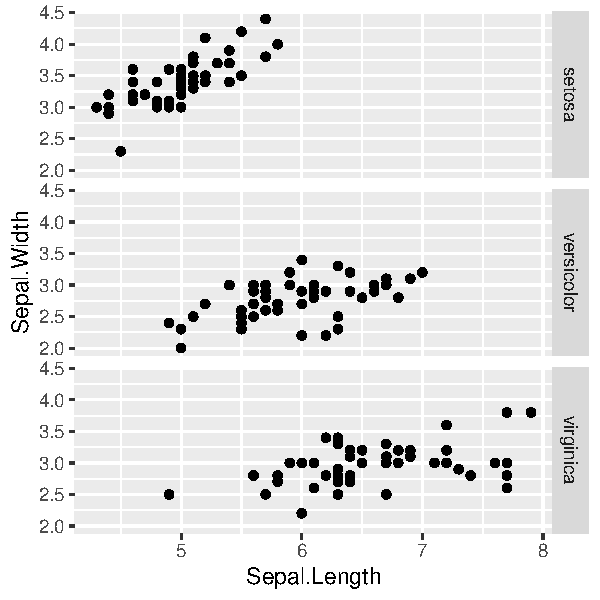
\includegraphics{Week3Answers_files/figure-latex/unnamed-chunk-17-1.pdf}
\caption{Scatterplot of sepal length and sepal width by species}
\end{figure}

\newpage

\hypertarget{patchwork-package-in-r}{%
\section{\texorpdfstring{\texttt{patchwork} package in
R}{patchwork package in R}}\label{patchwork-package-in-r}}

\begin{Shaded}
\begin{Highlighting}[]
\KeywordTok{library}\NormalTok{(patchwork) }
\end{Highlighting}
\end{Shaded}

First you need to assign a name for each graph. Here, I use \texttt{q1}
and \texttt{q2}.

\begin{Shaded}
\begin{Highlighting}[]
\NormalTok{q1 <-}\StringTok{ }\KeywordTok{qplot}\NormalTok{(}\DataTypeTok{x =}\NormalTok{ Species, }\DataTypeTok{y =}\NormalTok{ Sepal.Width, }\DataTypeTok{data =}\NormalTok{ iris, }\DataTypeTok{geom =} \KeywordTok{c}\NormalTok{(}\StringTok{"point"}\NormalTok{,}\StringTok{"jitter"}\NormalTok{,}\StringTok{"boxplot"}\NormalTok{), }
      \DataTypeTok{alpha =} \FloatTok{0.5}\NormalTok{, }\DataTypeTok{colour =}\NormalTok{ Species, }\DataTypeTok{main =} \StringTok{"Distribution of Sepal.Width"}\NormalTok{)}
\NormalTok{q2 <-}\StringTok{ }\KeywordTok{qplot}\NormalTok{(}\DataTypeTok{x =}\NormalTok{ Species, }\DataTypeTok{y =}\NormalTok{ Sepal.Length, }\DataTypeTok{data =}\NormalTok{ iris, }\DataTypeTok{geom =} \KeywordTok{c}\NormalTok{(}\StringTok{"point"}\NormalTok{,}\StringTok{"jitter"}\NormalTok{,}\StringTok{"boxplot"}\NormalTok{), }
      \DataTypeTok{alpha =} \FloatTok{0.5}\NormalTok{, }\DataTypeTok{colour =}\NormalTok{ Species, }\DataTypeTok{main =} \StringTok{"Distribution of Sepal.Length"}\NormalTok{)}
\end{Highlighting}
\end{Shaded}

\hypertarget{arrange-multiple-graphs-row-wise-use}{%
\subsection{Arrange multiple graphs row-wise use
``/''}\label{arrange-multiple-graphs-row-wise-use}}

\begin{Shaded}
\begin{Highlighting}[]
\NormalTok{q1}\OperatorTok{/}\NormalTok{q2}
\end{Highlighting}
\end{Shaded}

\begin{figure}
\centering
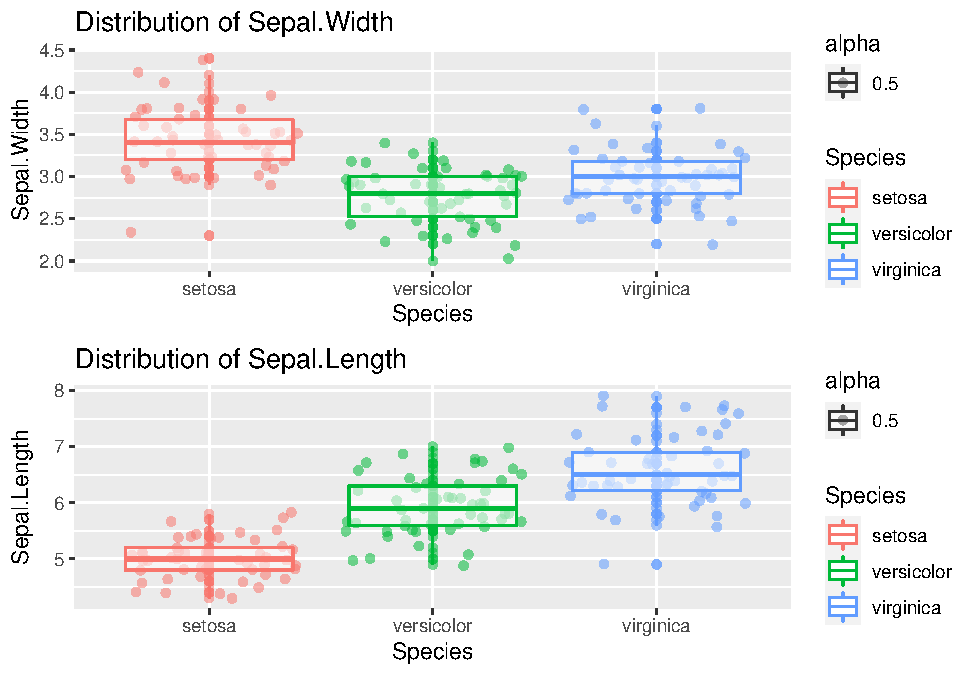
\includegraphics{Week3Answers_files/figure-latex/unnamed-chunk-20-1.pdf}
\caption{Arrange multiple graphs row-wise}
\end{figure}

\newpage

\hypertarget{arrange-multiple-graphs-column-wise-use}{%
\subsection{Arrange multiple graphs column-wise: use
``\textbar{}''}\label{arrange-multiple-graphs-column-wise-use}}

\begin{Shaded}
\begin{Highlighting}[]
\NormalTok{q1}\OperatorTok{|}\NormalTok{q2}
\end{Highlighting}
\end{Shaded}

\begin{figure}
\centering
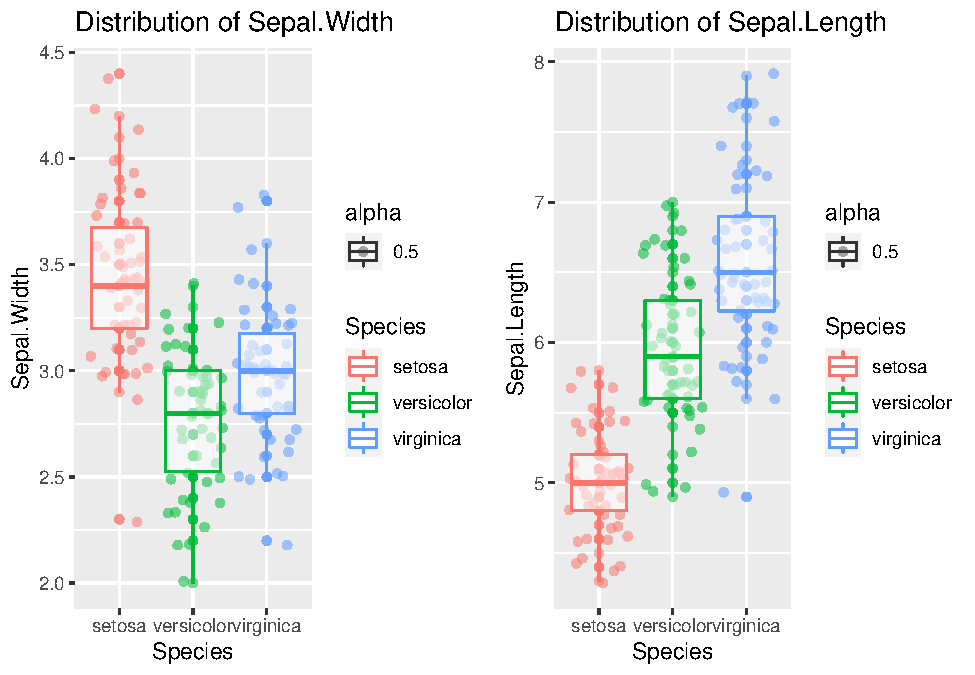
\includegraphics{Week3Answers_files/figure-latex/unnamed-chunk-21-1.pdf}
\caption{Arrange multiple graphs column-wise}
\end{figure}

\newpage

\hypertarget{arrange-multiple-graphs-both-row-wise-and-column-wise}{%
\subsection{Arrange multiple graphs both row-wise and
column-wise}\label{arrange-multiple-graphs-both-row-wise-and-column-wise}}

\begin{Shaded}
\begin{Highlighting}[]
\NormalTok{(q1}\OperatorTok{|}\NormalTok{q2)}\OperatorTok{/}\NormalTok{(q1}\OperatorTok{|}\NormalTok{q2)}
\end{Highlighting}
\end{Shaded}

\begin{figure}
\centering
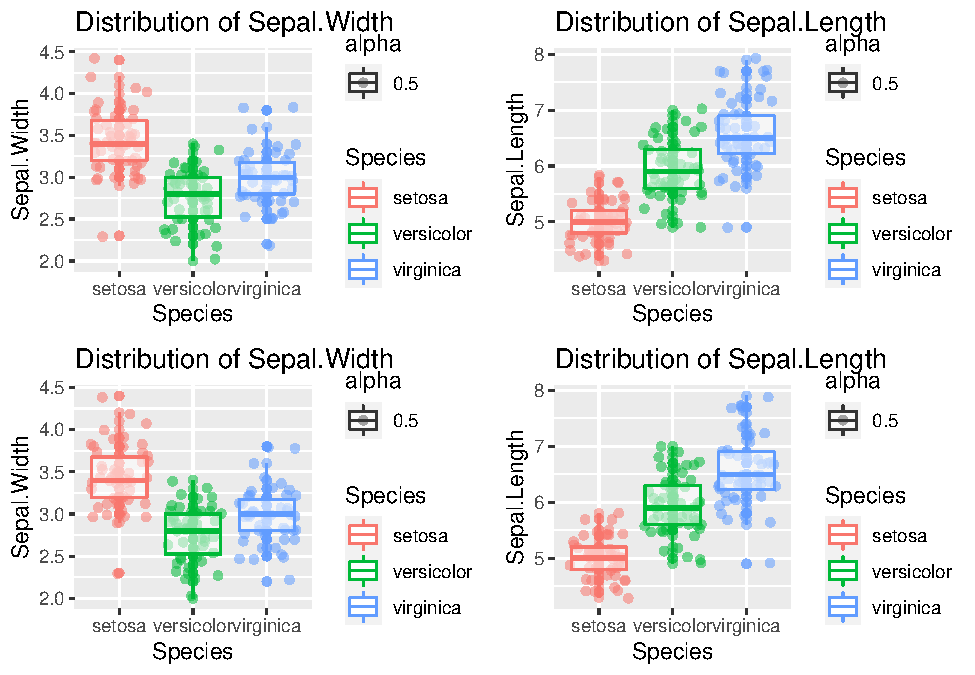
\includegraphics{Week3Answers_files/figure-latex/unnamed-chunk-22-1.pdf}
\caption{Arrange multiple graphs both row-wise and column-wise}
\end{figure}

\newpage

\hypertarget{stage-3-final-analysis}{%
\section{Stage 3: Final analysis}\label{stage-3-final-analysis}}

You do not need to include all the graphs to your final analysis. Please
select only the useful graphs which help you to tell the story in your
dataset. Here is mine.

\hypertarget{composition-of-the-sample}{%
\subsection{1. Composition of the
sample}\label{composition-of-the-sample}}

\begin{Shaded}
\begin{Highlighting}[]
\KeywordTok{qplot}\NormalTok{(}\DataTypeTok{x =}\NormalTok{ Species, }\DataTypeTok{data =}\NormalTok{ iris, }\DataTypeTok{geom =} \StringTok{"bar"}\NormalTok{, }\DataTypeTok{ylab =} \StringTok{"Count"}\NormalTok{, }
      \DataTypeTok{colour =}\NormalTok{ Species, }\DataTypeTok{fill =}\NormalTok{ Species,}
      \DataTypeTok{main =} \StringTok{"Composition of Species"}\NormalTok{)}
\end{Highlighting}
\end{Shaded}

\begin{figure}
\centering
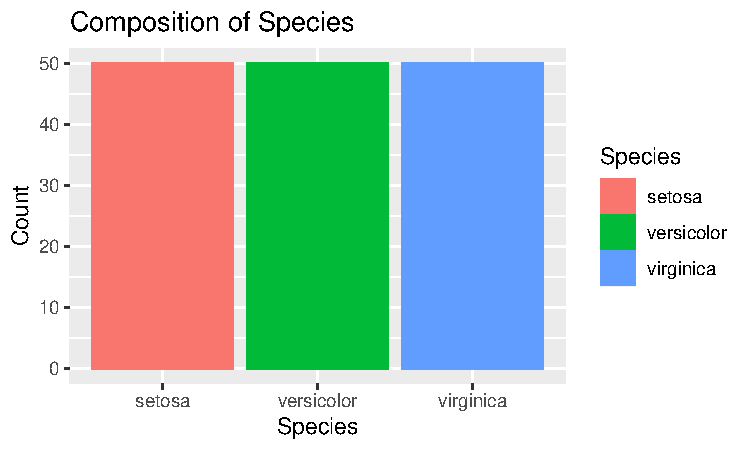
\includegraphics{Week3Answers_files/figure-latex/unnamed-chunk-23-1.pdf}
\caption{Composition of the sample}
\end{figure}

\newpage

\hypertarget{distribution-of-the-features-of-sepal-and-petal-by-species}{%
\subsection{2. Distribution of the features of sepal and petal by
species}\label{distribution-of-the-features-of-sepal-and-petal-by-species}}

\begin{Shaded}
\begin{Highlighting}[]
\NormalTok{q1 <-}\StringTok{ }\KeywordTok{qplot}\NormalTok{(}\DataTypeTok{x =}\NormalTok{ Species, }\DataTypeTok{y =}\NormalTok{ Sepal.Width, }\DataTypeTok{data =}\NormalTok{ iris, }\DataTypeTok{geom =} \KeywordTok{c}\NormalTok{(}\StringTok{"point"}\NormalTok{,}\StringTok{"jitter"}\NormalTok{,}\StringTok{"boxplot"}\NormalTok{), }
      \DataTypeTok{alpha =} \FloatTok{0.5}\NormalTok{, }\DataTypeTok{colour =}\NormalTok{ Species, }\DataTypeTok{main =} \StringTok{"(a) Distribution of Sepal Width"}\NormalTok{)}
\NormalTok{q2 <-}\StringTok{ }\KeywordTok{qplot}\NormalTok{(}\DataTypeTok{x =}\NormalTok{ Species, }\DataTypeTok{y =}\NormalTok{ Sepal.Length, }\DataTypeTok{data =}\NormalTok{ iris, }\DataTypeTok{geom =} \KeywordTok{c}\NormalTok{(}\StringTok{"point"}\NormalTok{,}\StringTok{"jitter"}\NormalTok{,}\StringTok{"boxplot"}\NormalTok{), }
      \DataTypeTok{alpha =} \FloatTok{0.5}\NormalTok{, }\DataTypeTok{colour =}\NormalTok{ Species, }\DataTypeTok{main =} \StringTok{"(b) Distribution of Sepal Length"}\NormalTok{)}
\NormalTok{q3 <-}\StringTok{ }\KeywordTok{qplot}\NormalTok{(}\DataTypeTok{x =}\NormalTok{ Species, }\DataTypeTok{y =}\NormalTok{ Petal.Width, }\DataTypeTok{data =}\NormalTok{ iris, }\DataTypeTok{geom =} \KeywordTok{c}\NormalTok{(}\StringTok{"point"}\NormalTok{,}\StringTok{"jitter"}\NormalTok{,}\StringTok{"boxplot"}\NormalTok{), }
      \DataTypeTok{alpha =} \FloatTok{0.5}\NormalTok{, }\DataTypeTok{colour =}\NormalTok{ Species, }\DataTypeTok{main =} \StringTok{"(c) Distribution of Petal Width"}\NormalTok{)}
\NormalTok{q4 <-}\StringTok{ }\KeywordTok{qplot}\NormalTok{(}\DataTypeTok{x =}\NormalTok{ Species, }\DataTypeTok{y =}\NormalTok{ Petal.Length, }\DataTypeTok{data =}\NormalTok{ iris, }\DataTypeTok{geom =} \KeywordTok{c}\NormalTok{(}\StringTok{"point"}\NormalTok{,}\StringTok{"jitter"}\NormalTok{,}\StringTok{"boxplot"}\NormalTok{), }
      \DataTypeTok{alpha =} \FloatTok{0.5}\NormalTok{, }\DataTypeTok{colour =}\NormalTok{ Species, }\DataTypeTok{main =} \StringTok{"(d) Distribution of Petal Length"}\NormalTok{)}
\NormalTok{(q1}\OperatorTok{|}\NormalTok{q2)}\OperatorTok{/}\NormalTok{(q3}\OperatorTok{|}\NormalTok{q4)}
\end{Highlighting}
\end{Shaded}

\begin{figure}
\centering
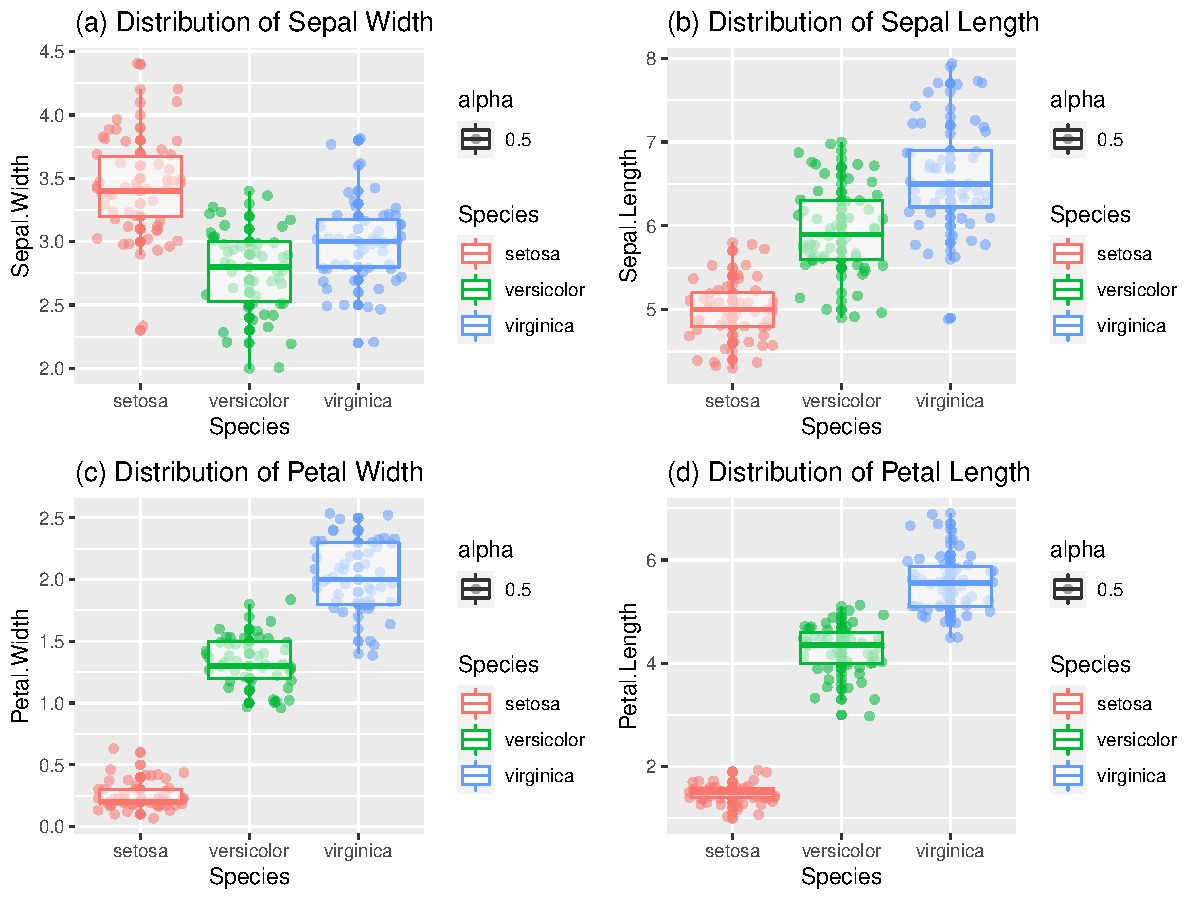
\includegraphics{Week3Answers_files/figure-latex/unnamed-chunk-24-1.pdf}
\caption{Distribution of features related to sepal and petal by species}
\end{figure}

\newpage

\hypertarget{relationship-between-features-of-sepal-and-petal-by-species}{%
\subsection{3. Relationship between features of sepal and petal by
species}\label{relationship-between-features-of-sepal-and-petal-by-species}}

\begin{Shaded}
\begin{Highlighting}[]
\NormalTok{p1 <-}\StringTok{ }\KeywordTok{qplot}\NormalTok{(}\DataTypeTok{x =}\NormalTok{ Sepal.Length, }\DataTypeTok{y =}\NormalTok{ Sepal.Width, }\DataTypeTok{data =}\NormalTok{ iris, }\DataTypeTok{geom =} \KeywordTok{c}\NormalTok{(}\StringTok{"point"}\NormalTok{,}\StringTok{"jitter"}\NormalTok{), }
      \DataTypeTok{alpha =} \FloatTok{0.5}\NormalTok{, }\DataTypeTok{colour =}\NormalTok{ Species, }
      \DataTypeTok{main=}\StringTok{"(a) Sepal Length and Sepal Width"}\NormalTok{)}
\NormalTok{p2 <-}\StringTok{ }\KeywordTok{qplot}\NormalTok{(}\DataTypeTok{x =}\NormalTok{ Petal.Length, }\DataTypeTok{y =}\NormalTok{ Petal.Width, }\DataTypeTok{data =}\NormalTok{ iris, }\DataTypeTok{geom =} \KeywordTok{c}\NormalTok{(}\StringTok{"point"}\NormalTok{,}\StringTok{"jitter"}\NormalTok{), }
      \DataTypeTok{alpha =} \FloatTok{0.5}\NormalTok{, }\DataTypeTok{colour =}\NormalTok{ Species, }
      \DataTypeTok{main =} \StringTok{"(b) Petal Length and Petal Width"}\NormalTok{)}
\NormalTok{p3 <-}\StringTok{ }\KeywordTok{qplot}\NormalTok{(}\DataTypeTok{x =}\NormalTok{ Sepal.Length, }\DataTypeTok{y =}\NormalTok{ Petal.Length, }\DataTypeTok{data =}\NormalTok{ iris, }\DataTypeTok{geom =} \KeywordTok{c}\NormalTok{(}\StringTok{"point"}\NormalTok{,}\StringTok{"jitter"}\NormalTok{), }
      \DataTypeTok{alpha =} \FloatTok{0.5}\NormalTok{, }\DataTypeTok{colour =}\NormalTok{ Species, }
      \DataTypeTok{main =} \StringTok{"(c) Sepal Length and Petal Length"}\NormalTok{)}
\NormalTok{p4 <-}\StringTok{ }\KeywordTok{qplot}\NormalTok{(}\DataTypeTok{x =}\NormalTok{ Sepal.Length, }\DataTypeTok{y =}\NormalTok{ Petal.Width, }\DataTypeTok{data =}\NormalTok{ iris, }\DataTypeTok{geom =} \KeywordTok{c}\NormalTok{(}\StringTok{"point"}\NormalTok{,}\StringTok{"jitter"}\NormalTok{), }
      \DataTypeTok{alpha =} \FloatTok{0.5}\NormalTok{, }\DataTypeTok{colour =}\NormalTok{ Species, }
      \DataTypeTok{main =} \StringTok{"(d) Sepal length and Petal Width"}\NormalTok{)}
\NormalTok{(p1}\OperatorTok{|}\NormalTok{p2)}\OperatorTok{/}\NormalTok{(p3}\OperatorTok{|}\NormalTok{p4)}
\end{Highlighting}
\end{Shaded}

\begin{figure}
\centering
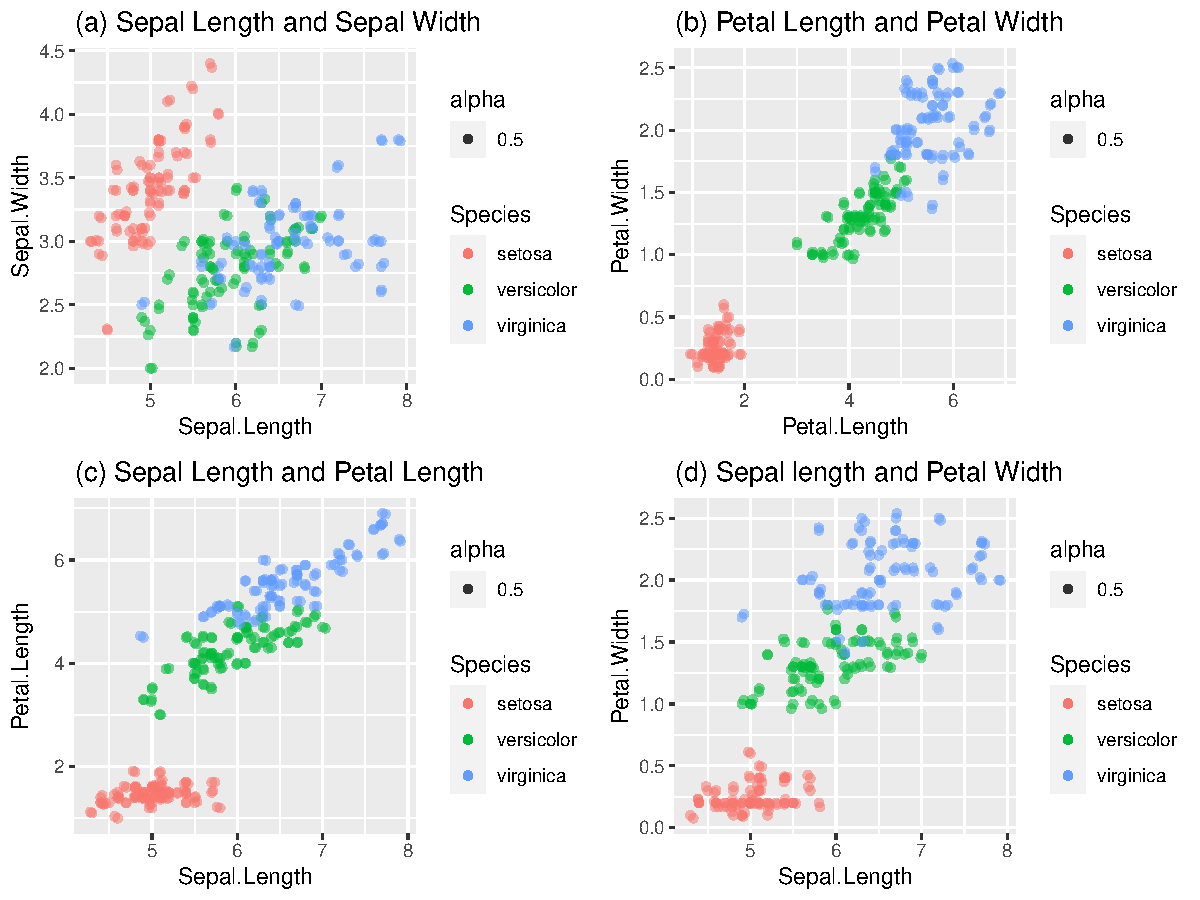
\includegraphics{Week3Answers_files/figure-latex/unnamed-chunk-25-1.pdf}
\caption{Relationship between features of sepal and petal by species}
\end{figure}

\textbf{Note: Interpret all figures in your final analysis.}

\end{document}
